\documentclass{jarticle}
\usepackage[dvipdfmx]{graphicx}
\usepackage{listings,jlisting,url,here}

\lstset{%
  language={C},
  basicstyle={\small},%
  identifierstyle={\small},%
  commentstyle={\small\itshape},%
  keywordstyle={\small\bfseries},%
  ndkeywordstyle={\small},%
  stringstyle={\small\ttfamily},
  frame={tb},
  breaklines=true,
  columns=[l]{fullflexible},%
  numbers=left,%
  xrightmargin=0zw,%
  xleftmargin=3zw,%
  numberstyle={\scriptsize},% stepnumber=1,
  numbersep=1zw,%
  lineskip=-0.5ex%
}


\title{28班 企画書}
\author{織田武瑠, 矢野大暉, 山口力也}
\date{2019/10/28 提出}

\begin{document}
\maketitle

\section{ゲーム内容}
\subsection{ゲームのタイトル}
エージェント3

\subsection{ジャンル}
脱出ゲーム

\subsection{概略}
ゲームの設定は,「犯罪組織に盗まれた金塊を組織に潜入して,複数のプレイヤーと協力して,組織的に取り返す」といった設定である.
本ゲームは,同一のサーバに接続した複数のプレイヤーが協力する脱出ゲームである.プレイヤーは出入り口からスタートし,敵キャラ(敵),監視カメラに見つからないように,ステージ上に設置された金塊をゲットし再び敵,監視カメラに見つからないように出入り口に帰ってくるゲームである.
ステージは複数用意されており,ステージが上がるごとに敵や監視カメラを増やすことで難易度を向上させる.

プレイヤーは敵キャラや監視カメラに対して妨害を行うことで,他プレイヤーが金塊を取るためのアシストを行うことができる.
プレイヤーが行うことができる妨害として以下が挙げられる.
\begin{itemize}
\item 敵キャラに話しかける → 敵の視界の固定
\item 監視カメラのハッキング → 監視が一時的に停止
\item 敵キャラに催涙スプレー → 敵の視界が無効化
\end{itemize}

\subsection{プレイ人数}
3人

\subsection{操作方法}
本ゲームはジョイパッドでの操作を行う.


移動 : ジョイパッドのアナログスティック\\
妨害アクション : 3ボタン\\
金塊を取得 : 4ボタン\\


\subsection{画面構成}
ゲームのイメージ図を図\ref{fig:gameimg}に示す.

\begin{figure}[H]
\begin{center}
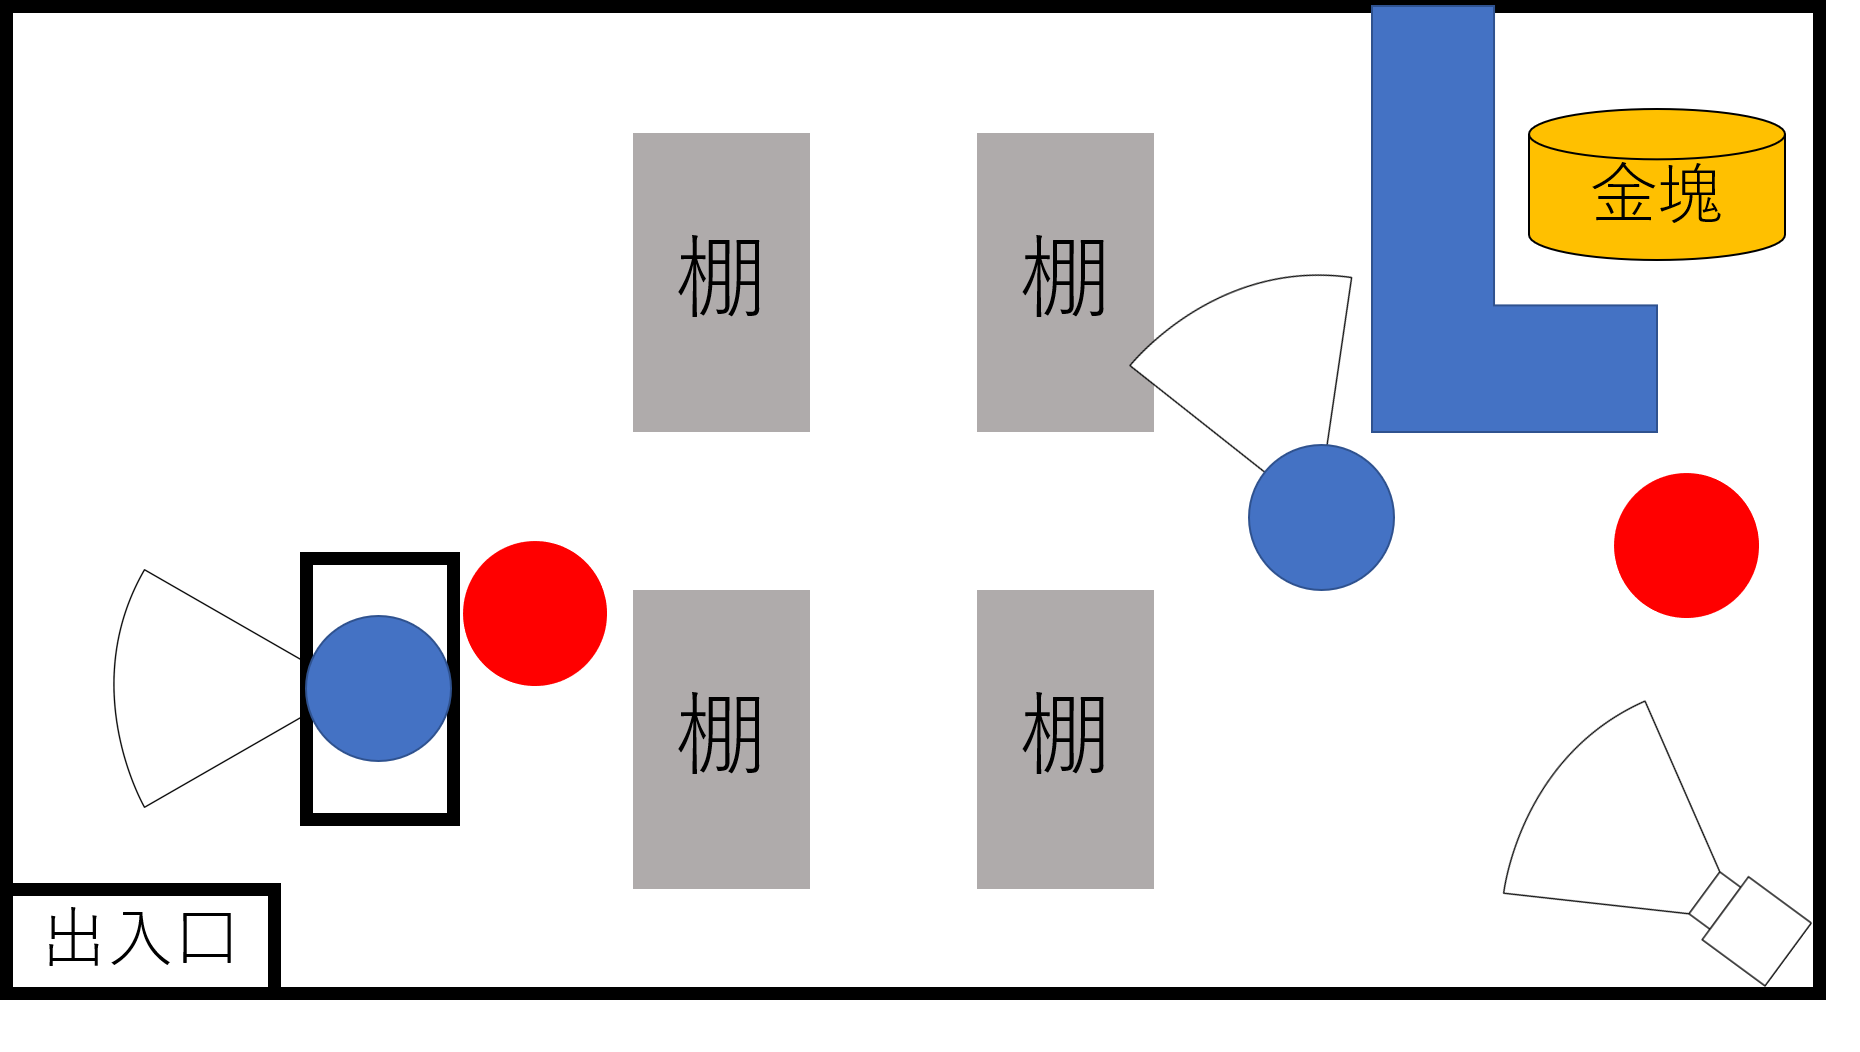
\includegraphics[width=\linewidth]{./zu/gamewindow.png}
\caption{ゲームウィンドウのイメージ}
\label{fig:gameimg}
\end{center}
\end{figure}

赤で示しているのがプレイヤー,青で示しているのが敵キャラ(敵),右下隅の物体が監視カメラである.
敵キャラ,監視カメラの扇形の物体は視界を表しており,この中にプレイヤーがいるとプレイヤーが「見つかった」判定となる.

\subsection{勝敗,クリア,終了条件}
クリア条件は,プレイヤーが金塊を取って出入り口へ向かうことができればゲームクリアである.
ゲームオーバー条件はプレイヤーが敵キャラまたは監視カメラに見つかってしまうことである.

\subsection{その他の特徴}
敵キャラの動きはルールベース型AIを採用している.進捗状況によっては,強化学習なども用いる.
敵キャラのAIの具体例としては以下が挙げられる.
\begin{itemize}
\item 敵がプレイヤーに近づく → 敵がプレイヤーの方向へ向く
\item 監視カメラにプレイヤーが近づく → カメラの首振りのスピードがはやくなる
\end{itemize}

また,ゲームに使用する素材はオリジナルのものを作成する.

\section{実装方法:データの構造}
\subsection{ゲームに必要な変数,構造体}

\begin{table}[H]
\begin{tabular}{|r|l|l|}
\hline
\multicolumn{3}{|l|}{共通の構造}       \\ \hline
データ型           & 変数名  	& 内容        \\ \hline
SDL\_Rect            & chararect & キャラクターの座標,高さ,幅  \\
int & speed   & キャラクターの速度 \\
SDL\_Texture*					 & imgaddress	& キャラクターの参照する画像のアドレス \\ \hline
\end{tabular}
\end{table}

\begin{table}[H]
\begin{tabular}{|r|l|l|}
\hline
\multicolumn{3}{|l|}{プレイヤーの構造}       \\ \hline
データ型           & 変数名  	& 内容        \\ \hline
SDL\_Bool		&	isgetgold	& プレイヤーが金塊を持っているかどうか\\ \hline
\end{tabular}
\end{table}

\begin{table}[H]
\begin{tabular}{|r|l|l|}
\hline
\multicolumn{3}{|l|}{敵キャラの構造}       \\ \hline
データ型           & 変数名  	& 内容        \\ \hline
SDL\_Bool		&	isfoundplayer	& 敵キャラがプレイヤーを発見したかどうか\\ \hline
\end{tabular}
\end{table}

\begin{table}[H]
\begin{tabular}{|r|l|l|}
\hline
\multicolumn{3}{|l|}{監視カメラの構造}       \\ \hline
データ型           & 変数名  	& 内容        \\ \hline
int		&	speed	& 監視カメラの首振りのスピード\\ \hline
\end{tabular}
\end{table}




\section{実装方法:モジュール}
\subsection{ゲームに必要な関数等の説明}

\begin{table}[H]
\begin{tabular}{|r|l|}
\hline
\multicolumn{2}{|l|}{void StartUp(void)}       \\ \hline
関数名           & StartUp \\ \hline
機能     & SDLなどの初期化処理を行う関数  \\
引数 	 	 & なし \\
返り値	 & なし \\ \hline
\end{tabular}
\end{table}


\begin{table}[H]
\begin{tabular}{|r|l|}
\hline
\multicolumn{2}{|l|}{void Destroy(void)}       \\ \hline
関数名           & Destroy \\ \hline
機能     & SDLなどの終了処理を行う関数  \\
引数 	 	 & なし \\
返り値	 & なし \\ \hline
\end{tabular}
\end{table}


\begin{table}[H]
\begin{tabular}{|r|l|}
\hline
\multicolumn{2}{|l|}{void PlayerSystem(void)}       \\ \hline
関数名           & PlayerSystem\\ \hline
機能     &  プレイヤーの移動などの処理を行う  \\
引数 	 	 & なし \\
返り値	 & なし \\ \hline
\end{tabular}
\end{table}


\begin{table}[H]
\begin{tabular}{|r|l|}
\hline
\multicolumn{2}{|l|}{void EnemySystem(void)}       \\ \hline
関数名           &  EnemySystem \\ \hline
機能     & 敵キャラの移動などの処理を行う  \\
引数 	 	 & なし \\
返り値	 & なし \\ \hline
\end{tabular}
\end{table}


\begin{table}[H]
\begin{tabular}{|r|l|}
\hline
\multicolumn{2}{|l|}{void CameraSystem(void)}       \\ \hline
関数名           & CameraSystem  \\ \hline
機能     & カメラの座標などの変更を行う  \\
引数 	 	 & なし \\
返り値	 & なし \\ \hline
\end{tabular}
\end{table}

\begin{table}[H]
\begin{tabular}{|r|l|}
\hline
\multicolumn{2}{|l|}{void Collision(void)}       \\ \hline
関数名           & Collision  \\ \hline
機能     & 衝突判定を行う関数  \\
引数 	 	 & なし \\
返り値	 & なし \\ \hline
\end{tabular}
\end{table}

\begin{table}[H]
\begin{tabular}{|r|l|}
\hline
\multicolumn{2}{|l|}{void RenderWindow(void)}       \\ \hline
関数名           & RenderWindow  \\ \hline
機能     & 画面の描画を行う関数  \\
引数 	 	 & なし \\
返り値	 & なし \\ \hline
\end{tabular}
\end{table}


\section{ガントチャート}
作成したガントチャートを図\ref{fig:gunt}に示す.

\begin{figure}[H]
\begin{center}
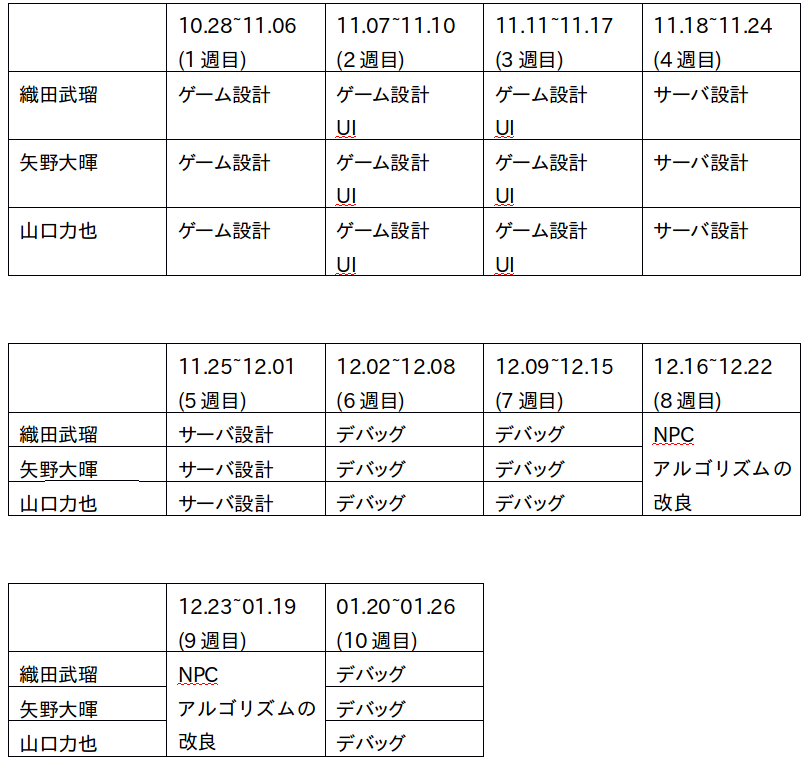
\includegraphics[width=\linewidth]{./zu/gunt.png}
\caption{ガントチャート}
\label{fig:gunt}
\end{center}
\end{figure}



\end{document}
